\section{Impact on the signal}

\subsection{Jet selection accuracy}

\def\figDir{figures/pairAGraph/SMNR_mc16a_PFlow-APR2020-5jets/}

%\begin{figure}
%\includegraphics[width=\textwidth]{{\figDir/}}
%\end{figure}


\subsection{Cases where pairAGraph got the correct jets and the baseline selected the wrong jets}

% 4b exs:
% Evt 1513
% Evt 1687

\def\subDir{SM_2b/eventDisplays/pagJetSelRight/}

\begin{figure}
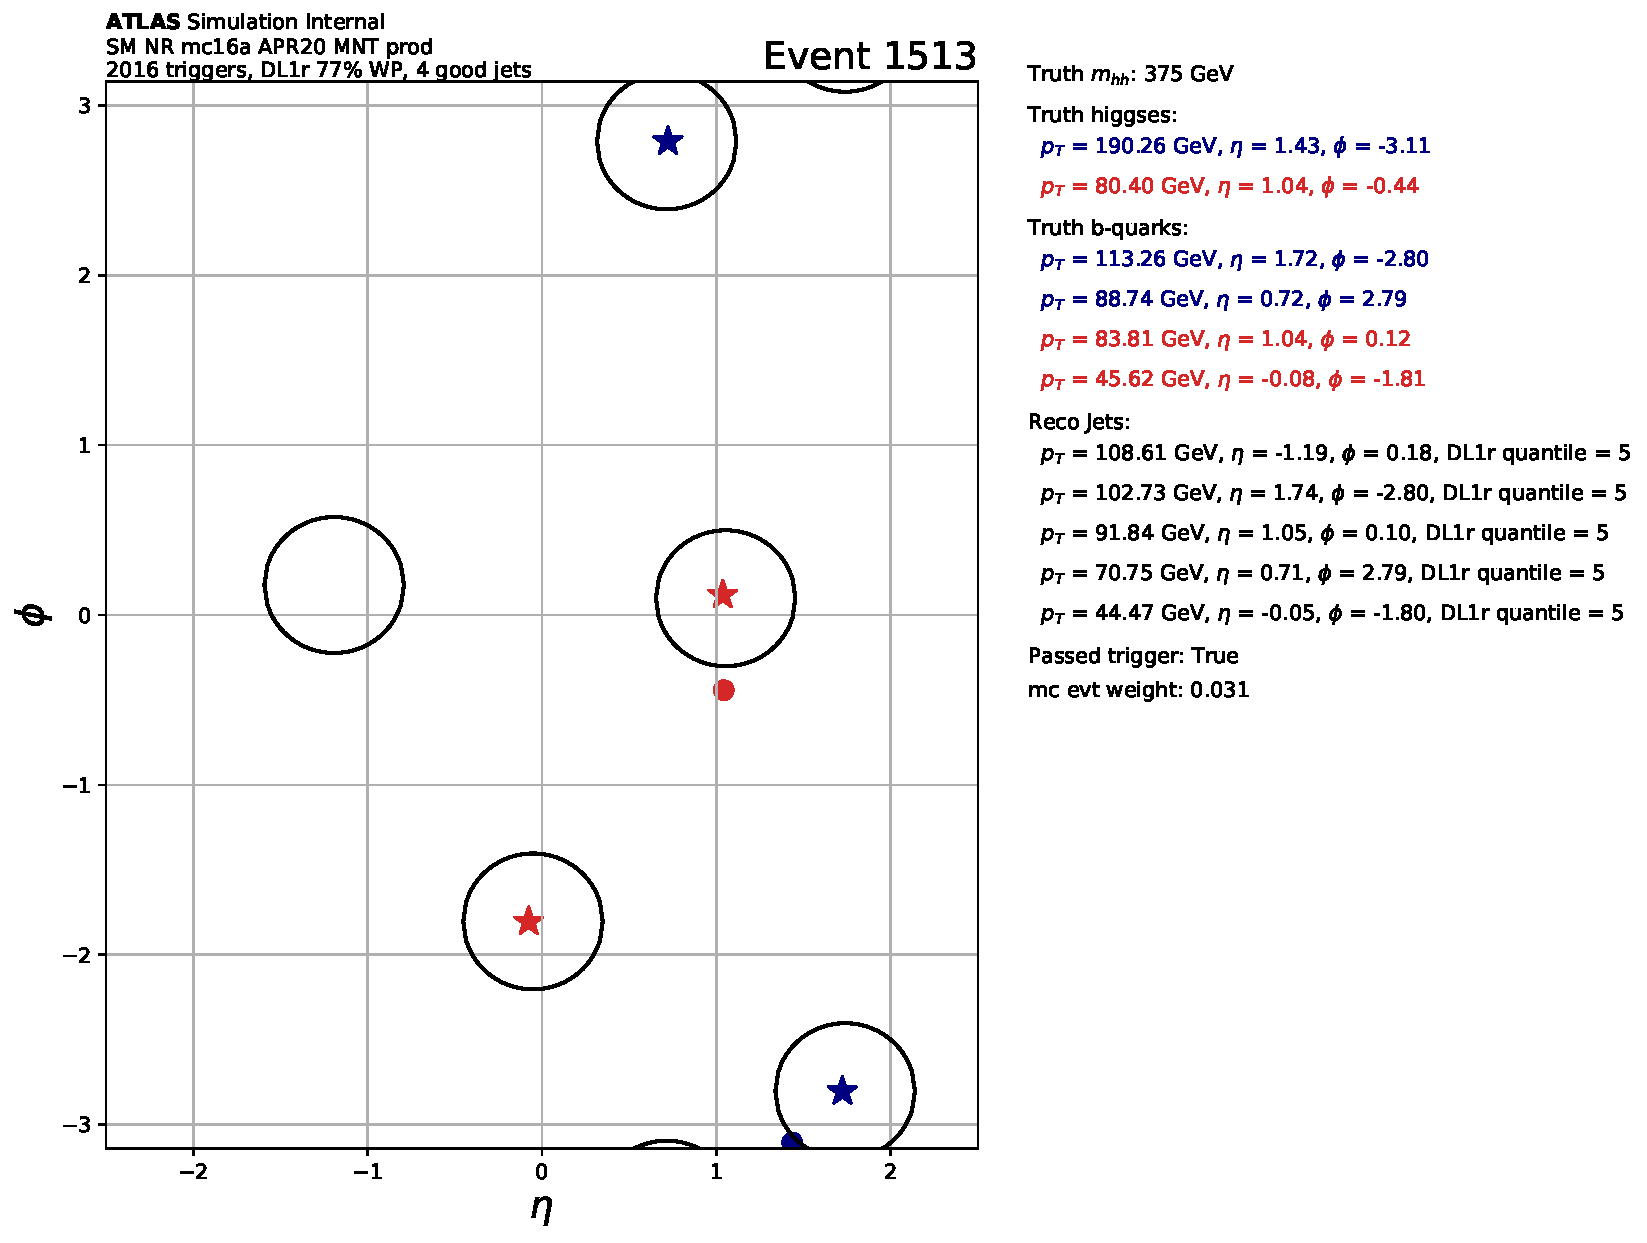
\includegraphics[width=\textwidth]{{\figDir/\subDir/evt_1513.pdf}}
\end{figure}

\begin{figure}
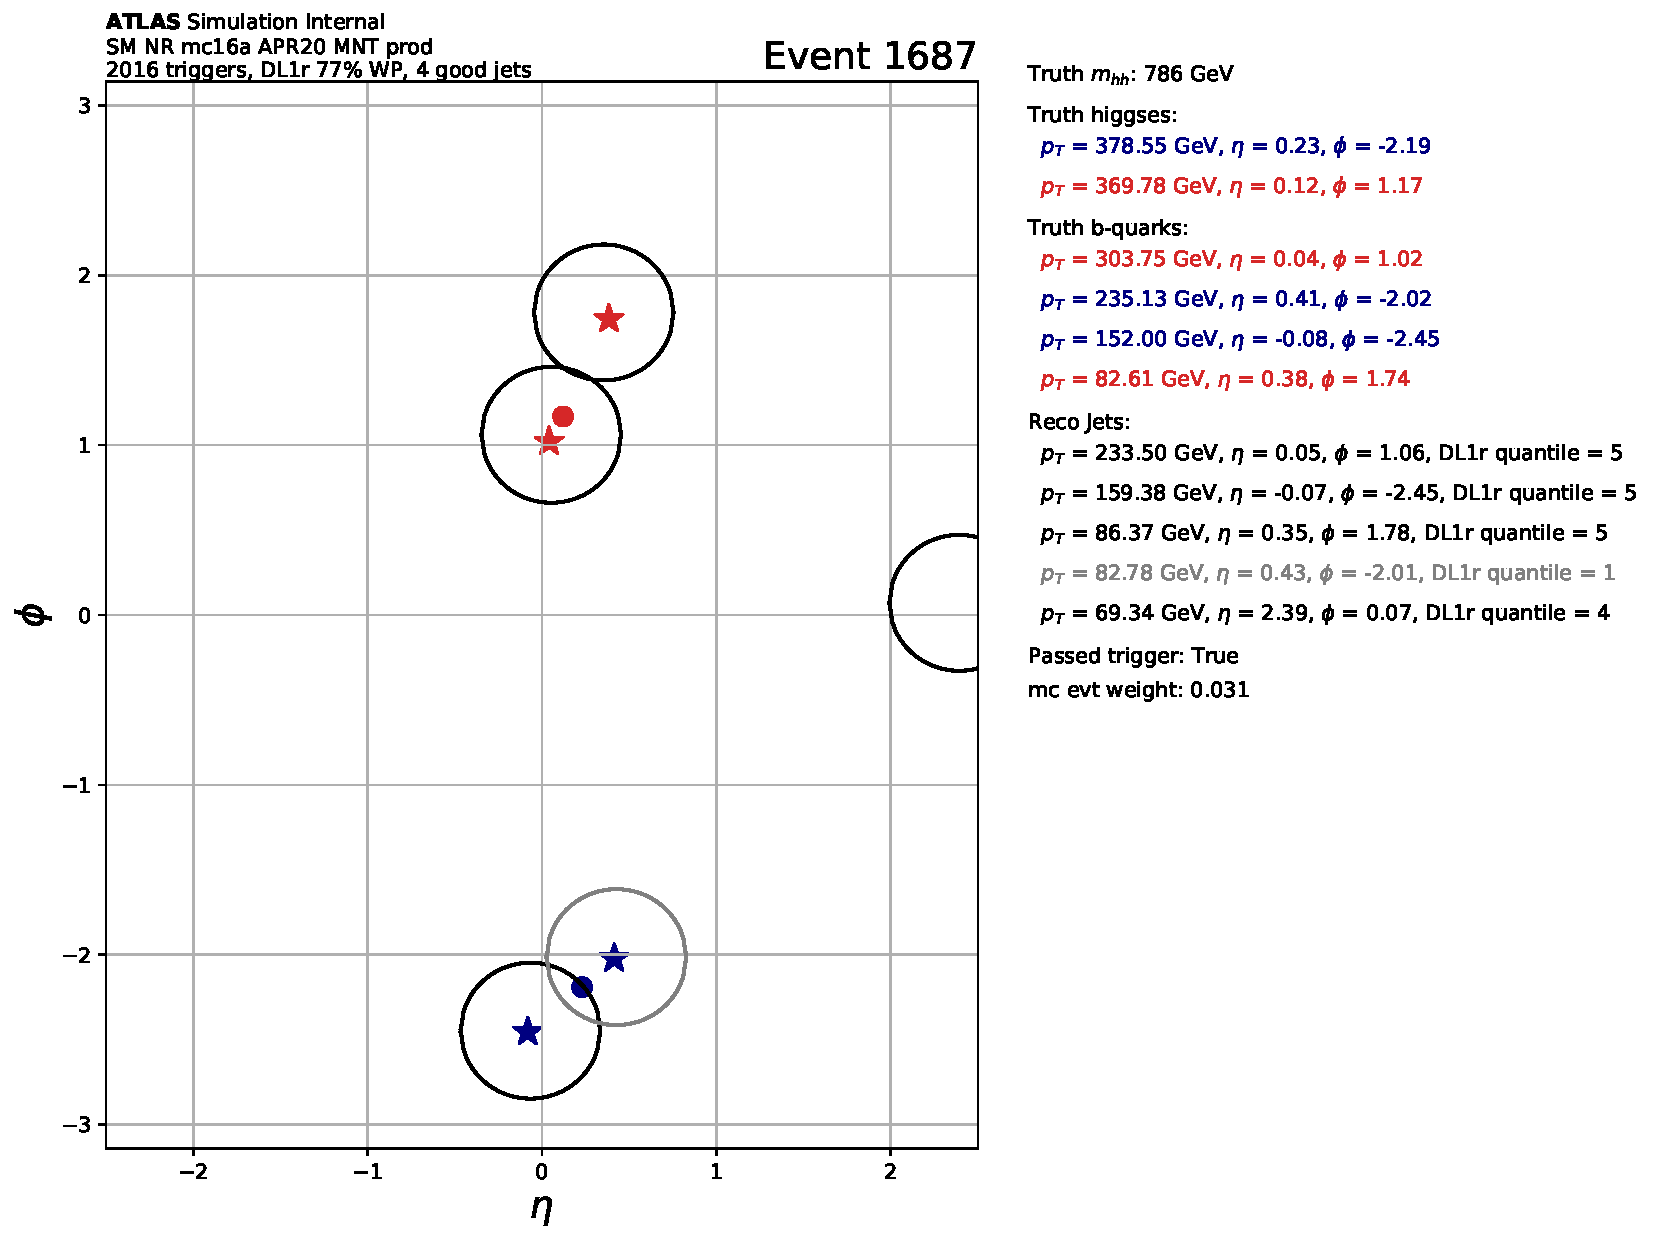
\includegraphics[width=\textwidth]{\figDir/\subDir/evt_1687}
\end{figure}

%\subsectio{How often does}

\subsection{What extra information was pairAGraph learning?}

RECOIL (need plot)

Oh - also I'll need to decide if I just want to show 4b or the 3b cats too!

\begin{figure}
\centering
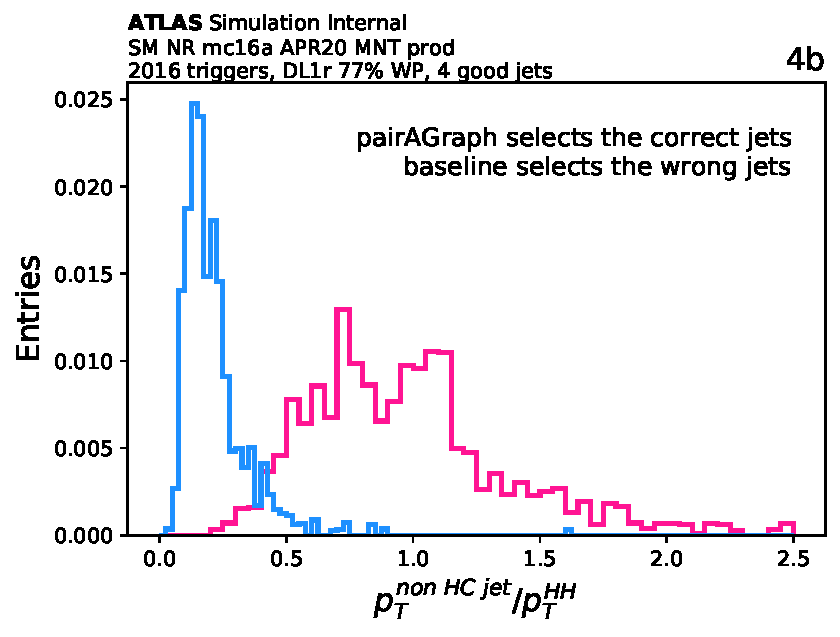
\includegraphics[width=.75\textwidth]{{\figDir/SM_2b/pt_recoil_pt_4j_base_4b.pdf}}
\caption{\hl{need to add a legend!!}}
\end{figure}


\begin{figure}
\subfloat{
	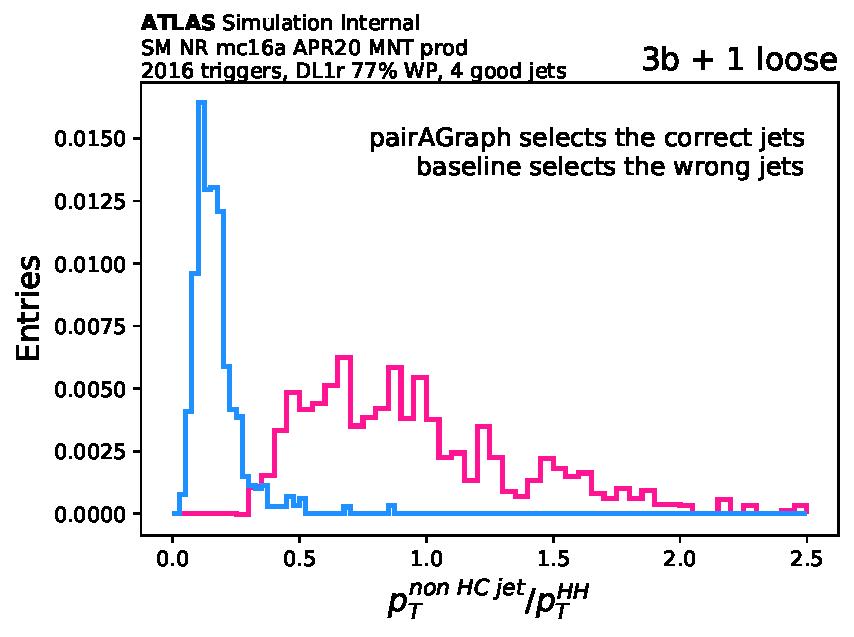
\includegraphics[width=.44\textwidth]{{\figDir/SM_2b/pt_recoil_pt_4j_base_3b1loose.pdf}}
}
\subfloat{
	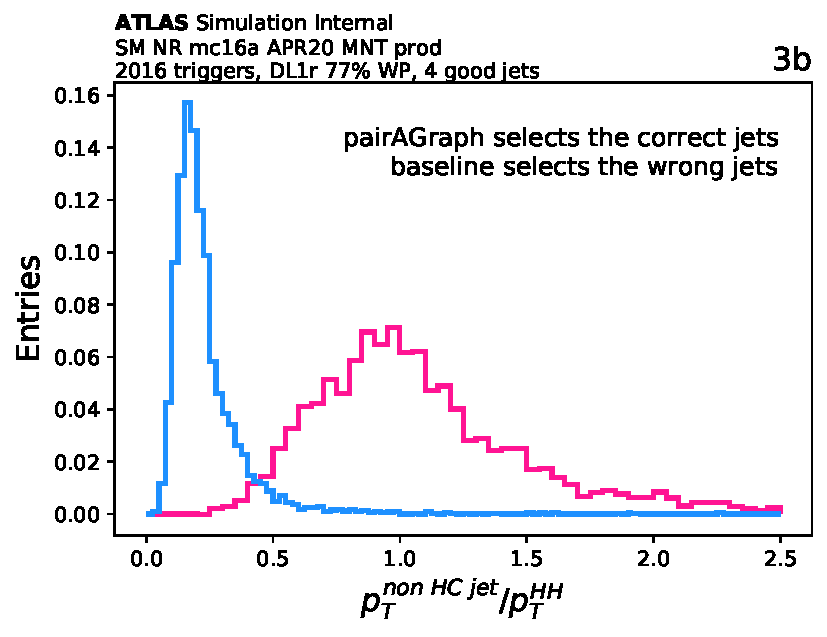
\includegraphics[width=.44\textwidth]{{\figDir/SM_2b/pt_recoil_pt_4j_base_3b.pdf}}
}
\caption{\hl{need to add a legend!!}}
\end{figure}


%\FloatBarrier
%\clearpage

\subsection{Pairing accuracy}

\begin{table}[htbp]
	\centering
	\begin{adjustbox}{width=\columnwidth,center}
	\begin{tabular}{ c | c | c | c | c | c | c  }
	{Pairing algorithm} & {\bfseries Pairing} & {\bfseries MDR } & {\bfseries MDpT} & {\bfseries $\Delta \eta_{HH} < 1.5$} & {\bfseries $X_{Wt} > 1.5$} & { \bfseries SR} \\
	\hline\hline
	\textcolor{green}{MDR + min(Dhh)} & 71.8\% & 79.7\% & 79.7\% & 80.1 \% & 83.3 \% & 93.6 \% \\
	\textcolor{orange}{$min\left(\Delta R_{jj}^{HC \ 1} \right)$} & 69.7 \^ & -- & 73.7 \% & 74.0 \% & 78.4\% & 94.7\% \\
	\textcolor{hh:darkpink}{pairAGraph train SM} & 78.4 \% & -- & -- & 79.6 \% & 82.4 \% & 94.2\% \\
	\textcolor{hh:medturquoise}{pairAGraph train $\kappa_\lambda = 10$} & 76.8\% & -- & -- & 78.4 \% &81.3 \% & 94.1 \% \\
	\hline
	\end{tabular}
	\end{adjustbox}
	\caption{Cuts are applied sequentially from the left to the right.}
	\label{tab:rw-inputs}
\end{table}

\textbf{Observation \# 1: The ``after pairing'' column} 

\textbf{Observartion \# 2: Applying the cuts sequentially}

\textbf{Observation \# 3: Inside of the SR}



\subsection{Visualization of the attention weights}

One of the attractive features of using a transformer architecture was that the multi-head attention mechanism in the 


\def\figDir{figures/pairAGraph/SMNR_mc16a_PFlow-AUG2019-5jets/graphViz}

\begin{figure}[hbt]
	\centering
	\subfloat{
		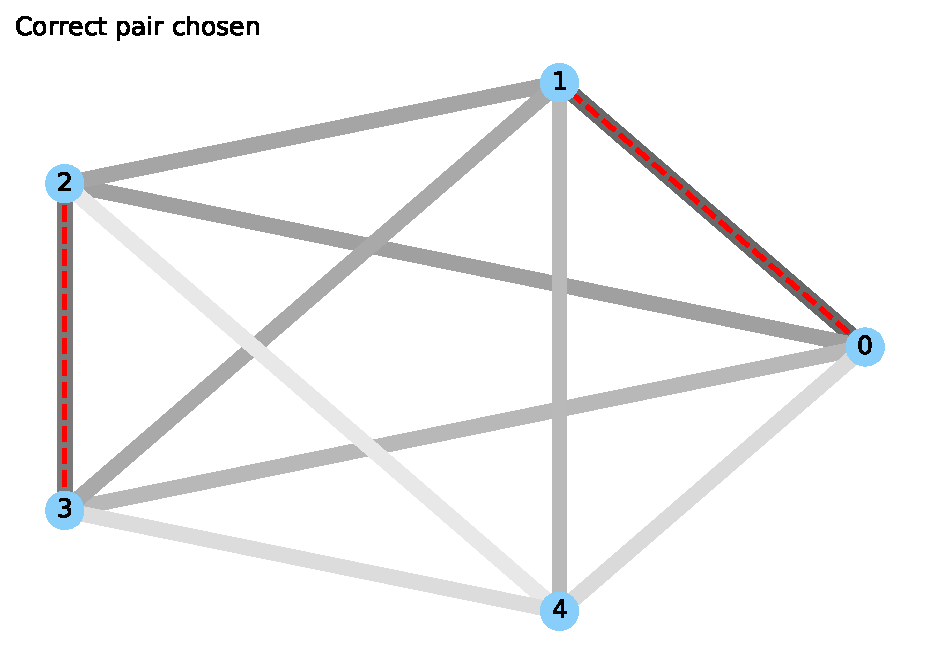
\includegraphics[width=.33\textwidth]{{\figDir/graph_5jets_0}}
	}
	\subfloat{
		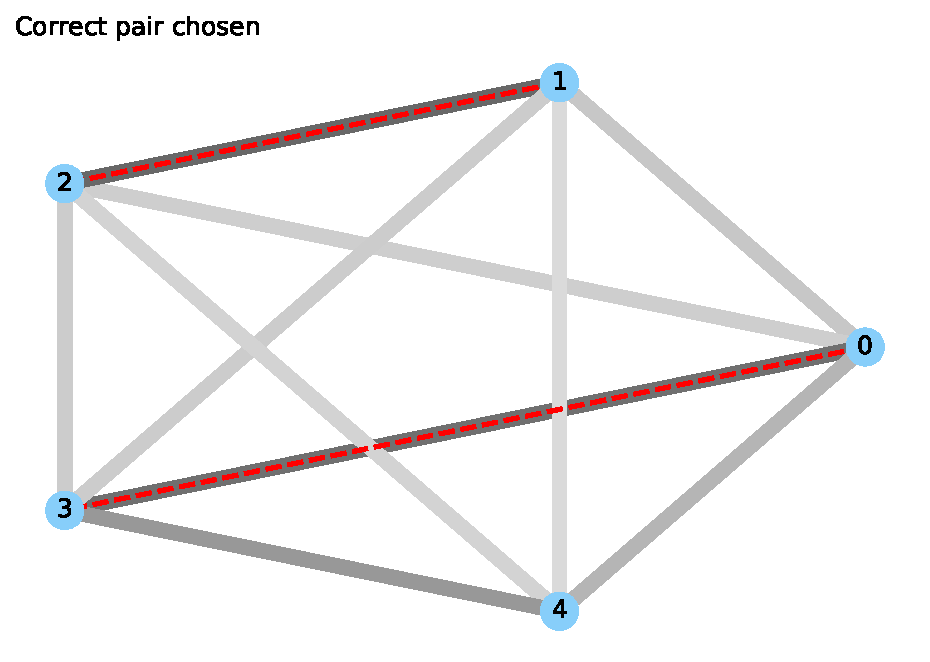
\includegraphics[width=.33\textwidth]{{\figDir/graph_5jets_2}}
	}
	\subfloat{
		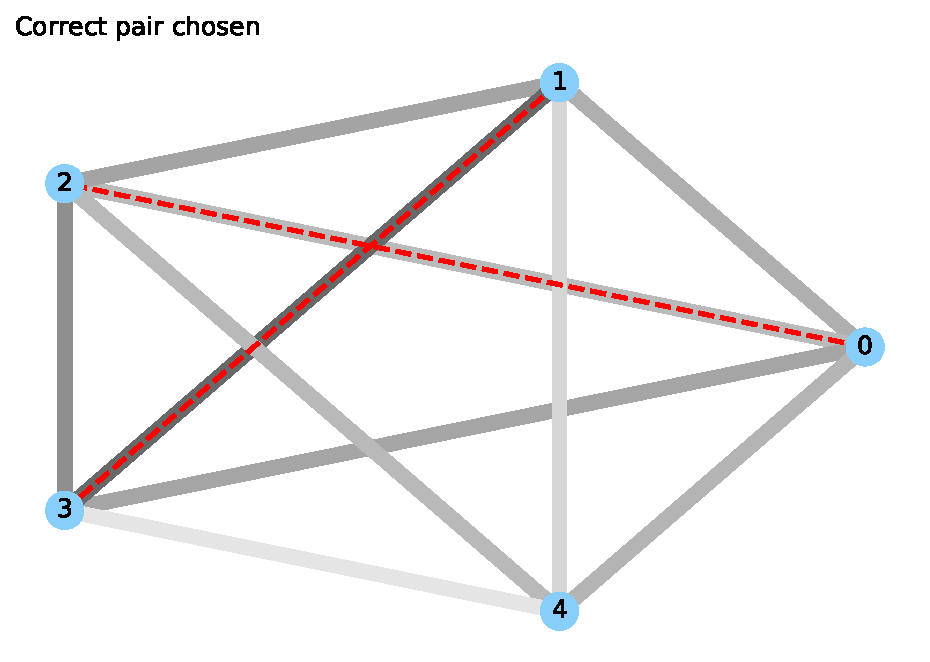
\includegraphics[width=.33\textwidth]{{\figDir/graph_5jets_3}}
	}
	\caption{Visualization of the multi-head attention weights from the transformer. The circles on the graph}
\end{figure}
% note: event 15 looks quite wierd, but I think this is because I was visualizing the attention weights, not the final jet similarity matrix


